% !TEX root = ./main.tex

\section{Foreword}

Imagine a mobile robot navigating a complex environment for the first
time.  Limited training data often hinders its ability to recognize
previously unseen locations. This challenge highlights the need for
robust visual place recognition (VPR) techniques in mobile robotics.
The fields of deep learning and mobile robotics are undergoing rapid
advancements, with a growing focus on developing more generalized
solutions. One promising approach involves \emph{foundation models},
capable of learning transferable representations from massive
datasets. These models are paving the way for tackling open-set
problems, where robots can excel even in scenarios not explicitly
encountered during training. This thesis investigates the potential of
foundation models to improve the perception capabilities of mobile
robots, focusing on the development of a novel VPR technique called
AnyLoc.

AnyLoc is a novel image retrieval system that leverages latent
features extracted by foundation models.  It employs aggregation
techniques to combine these features, resulting in robust place
descriptors crucial for accurate visual place recognition.

\subsection{Contribution}

This thesis, along with the publication supporting it (AnyLoc
\cite{Keetha2023AnyLocTU}), has the following content and 
contributions

\begin{itemize}
    \item \cref{ch:intro}: An overview of mobile robotics,
        Simultaneous Localization and Mapping (SLAM), and Visual Place
        Recognition (VPR) systems.
    \item \cref{ch:foundation-models}: An overview of foundation
        models: ViT architecture, training pipeline for
        self-supervised learning, and the backbone models for AnyLoc.
    \item \cref{ch:anyloc}: Proposes an image retrieval method,
        AnyLoc, that is a new state-of-the-art on various testing
        scenarios, yielding twice the performance of supervised VPR
        benchmarks. Interestingly, it looses no performance even after
        a \texttt{95x} reduction in descriptor size, which is
        \emph{unprecedented} in VPR.
    \item \cref{ch:conc}: Concludes this thesis with presenting
        solutions to current problems and some ideas for future
        development.
\end{itemize}

\section{Understanding the Area of Contribution}

This thesis introduces AnyLoc \cite{Keetha2023AnyLocTU}, a novel image
retrieval system that leverages features extracted from foundation
models and employs conventional aggregation techniques to create
robust place descriptors.  Image retrieval (IR) plays a crucial role
in various applications, including:

\begin{itemize}
    \item \emph{Visual Place Recognition} (VPR) in Mobile Robotics
        \cite{Humenberger2022InvestigatingTR}: VPR systems rely on IR
        to identify previously encountered locations, enabling tasks
        like navigation and loop closure within Simultaneous
        Localization and Mapping (SLAM). This is also the direction in
        which this thesis is oriented.
    \item Remote Sensing and \emph{Geographic Information Systems}
        (GIS) \cite{Maiwald2021FullyAP}: IR techniques are used to
        analyze and classify satellite or aerial imagery, aiding tasks
        like land cover change detection or identifying specific
        features in large datasets.
    \item \emph{Medical Image Retrieval} \cite{Qayyum2017MedicalIR, 
        Lehmann2004ContentbasedIR}: In healthcare, IR helps medical
        professionals retrieve relevant medical images (e.g., X-rays,
        MRIs) based on specific criteria, assisting in diagnosis and
        treatment planning.
    \item \emph{Content-based Image Search}
        \cite{Hermes2023ContentbasedIR}: IR powers search engines and
        applications that allow users to find similar images based on
        visual content, facilitating tasks like product identification
        or searching for visually similar items online and organizing
        a large album of unorganized photos.
\end{itemize}

The reminder of this chapter describes a mobile robotics system, parts
of a SLAM system (\cref{subsec:intro-loc-and-map}), a VPR system in
SLAM (\cref{subsec:intro-vpr}), and associated methods and jargon.
\cref{ch:foundation-models} introduces foundation models and related
concepts needed for this thesis. Our method, AnyLoc, is presented in
\cref{ch:anyloc}. We conclude with possible future directions in
\cref{ch:conc}.

\subsection{Mobile Robot Systems}
\label{subsec:intro-mobile-robotics}

\begin{figure}
    \centering
    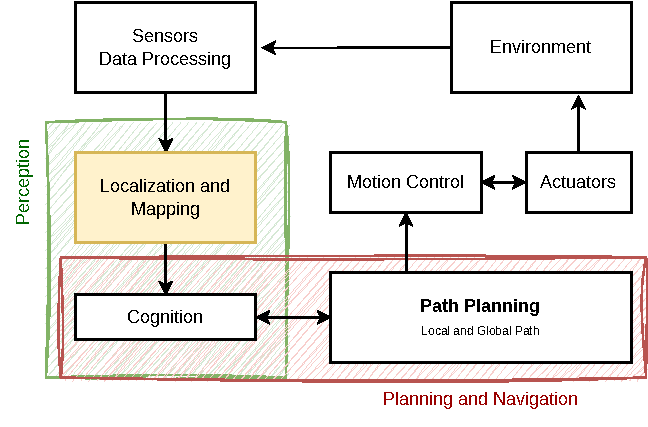
\includegraphics{robotic_systems_overview.pdf}
    \caption{Mobile Robotics System}
    \small
        The \emph{perception} stack makes sense of the environment and
        the \emph{planning and navigation} stack makes the robot
        navigate in the environment.
    \label{fig:mobile_robot_system}
\end{figure}

The software of mobile robots is composed of various modules. Most
systems comprise of the following parts (also highlighted in
\cref{fig:mobile_robot_system})

\begin{itemize}
    \item A \emph{data processing} module collects information from
        the environment through sensors and performs signal processing
        to get meaningful information.
    \item A \emph{localization and mapping} module creates and
        maintains a map of the environment (in which the robot can
        navigate). It also localizes the robot in that map (usually as
        a temporal pose sequence).
    \item A \emph{cognition} module transforms the map and robot poses
        into information that is needed for downstream tasks. For
        example: identifying obstacles and a goal for the task of
        navigating while avoiding obstacles.
    \item A \emph{path planning} module contains motion planners to
        guide the robot through the environment. Generally, they are
        comprised of local planners for immediate vicinity and global
        planners for high-level goals.
    \item A \emph{motion control} module is tightly coupled with
        \emph{actuators} which cause motion. It usually contains a
        motion model to estimate the actuation values.
\end{itemize}

The \emph{perception} stack consists of the localization and mapping
and the cognition module while the \emph{planning and navigation}
stack consists of the cognition module and the path planning module.
Note that the cognition module could share parts with the perception
and the planning and navigation stacks.

This thesis primarily focuses on parts of the \emph{localization and
mapping} module. A larger overview of mobile robot systems can be
found in \cite{Rubio2019ARO}. A more comprehensive study of various
aspects of mobile robotics can be found in
\cite{Choset2007PrinciplesOR} (for overview and background),
\cite{Thrun2005ProbabilisticR} (perception), \cite{Patle2019ARO}
(planning and navigation), \cite{Anish2017MobileRN} (navigation and
obstacle avoidance), and \cite{Featherstone2000RobotDE} (motion
control).

\subsection{Localization and Mapping}
\label{subsec:intro-loc-and-map}

Simultaneous Localization and Mapping (SLAM) is a type of localization
and mapping system where the location of the robot (agent) and the map
of the environment are jointly estimated. A review of different types
of visual SLAM algorithms can be found in \cite{Barros2022ACS,
Taketomi2017VisualSA, Cadena2016PastPA}.

\begin{figure}
    \centering
    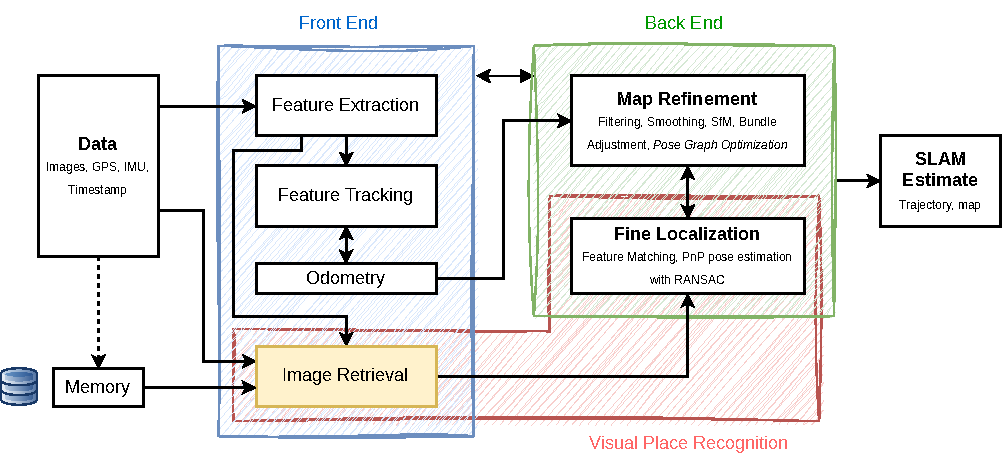
\includegraphics[width=\textwidth]{slam_systems.pdf}
    \caption{General SLAM Systems}
    \small
        The \emph{front end} module performs feature extraction,
        feature tracking, and gets the odometry of the robot. It also
        does coarse visual place recognition by image retrieval. The
        \emph{back end} module does fine localization (gets loop
        closures) and does map refinement. The map (containing the
        poses and the environment) is shared with both the modules.
    \label{fig:slam_system}
\end{figure}

This is conventionally achieved using system models and filtering
methods like Kalmann Filters (KF), Extended Kalman Filters (EKFs),
particle filters, etc. Most algorithms minimize a photometric
projection error to estimate the sensor's pose for a coarse
localization in the map. Lately, visual SLAM algorithms employ
optimization techniques on various timescales and loop closures across
various distances. A system of equations, projecting objects in the
map in camera frames, is solved to simultaneously obtain the camera
poses and map objects (usually like sparse point cloud). This is
formulated as an optimization problem on a graph of nodes
\cite{Grisetti2010ATO}.

A generic template for SLAM systems can be found in
\cref{fig:slam_system}. Most SLAM systems can be divided into two
parts

\begin{enumerate}
    \item A \emph{front end} module deals with all the data that
        enters the system. Common parts of it are centered around
        \begin{itemize}
            \item \emph{Feature extraction} where keypoint features
                are extracted from the images
            \item \emph{Feature tracking} where keypoints are tracked
                between consecutive images (to get relations)
            \item \emph{Odometry} which relates two consecutive poses
                (locations)
            \item \emph{Image Retrieval} where an agent can recognize
                a previously visited part of the map (stored in its
                memory). This gives a coarse location of a place the
                agent must have revisited.
        \end{itemize}
    \item A \emph{back end} module works on refining (optimizing) the
        map and other estimates (like trajectory). It usually consists
        of
        \begin{itemize}
            \item \emph{Fine Localization} where a more precise
                location of an image retrieval is estimated. This is
                usually done using PnP RANSAC techniques.
            \item \emph{Map Refinement} where the map estimates are
                fine tuned using optimizers. This is also called
                \emph{map optimization}.
        \end{itemize}
\end{enumerate}

This thesis primarily focuses on the Visual Place Recognition (VPR)
aspect of SLAM, which is further described in \cref{subsec:intro-vpr}.
The reminder of this subsection provides related details and a brief
overview of SLAM systems.

\subsubsection{Systems Similar to SLAM} 

Structure from Motion (SfM) aims to recover 3D geometry of a scene and
the camera poses from a set of 2D images. Bundle Adjustment (BA) aims
to refine the map and pose estimates through minimizing a reprojection
error. Indeed, SfM tools like COLMAP \cite{Schnberger2016PixelwiseVS,
Schnberger2016StructurefromMotionR} are used in SLAM systems as a
pre-processing tool. SLAM systems usually operate online (live, in
real-time). Maps used by SLAM systems are also capable of deeper
environment understanding.

Visual Odometry (VO) and similar mapping techniques aim to estimate
relative movement; SLAM aims to build a global and consistent map of
the environment while estimating pose. VO systems are prone to drift,
whereas SLAM systems correct drift through loop closures formed by the
visual place recognition module.


\subsubsection{Conventional SLAM Systems}

Some conventional SLAM systems are described hereon

\paragraph{MonoSLAM (2007) \cite{Davison2007MonoSLAMRS}} uses a known
target for initialization. The system's state vector is updated by
using a constant velocity model. Camera motion and environment
structure (map) are estimated using an Extended Kalman Filter (EKF).
The algorithm does not employ global optimization or loop closure
techniques.

\paragraph{PTAM (2007) \cite{Klein2007ParallelTA}} (Parallel Tracking
and Mapping) has two threads: tracking and mapping. The tracking
thread updates camera poses in the frames through feature search
(matching). The mapping thread performs data association, integration
of new frames, local and global bundle adjustment.

\paragraph{FAB-MAP (2008) \cite{Cummins2008FABMAPPL}} (FAst Binary
appearance-based Mapping) builds a map of visually similar locations
based on the environments appearance. The visual representations for
place recognition are built using a Bag-of-Words (BoW) representation
over image keypoint features. It incrementally builds and updates map
in a probabilistic framework.

\paragraph{DTAM (2011) \cite{Newcombe2011DTAMDT}} (Dense Tracking and
Mapping) has two parts (like PTAM but dense). The dense tracking
module estimates motion of camera by aligning a virtual camera in the
recorded map. The dense mapping module estimates the (inverse) depth
values of images by jointly minimizing the photometric error.

\paragraph{FAB-MAP 2.0 (2011) \cite{Cummins2011AppearanceonlySA}}
builds on FAB-MAP with a sparse approximation to the model, thus
allowing deployment on a much larger scale.

\paragraph{SVO (2014) \cite{Forster2014SVOFS}} (Semi-Direct Visual
Odometry) minimizes the photometric error and performs feature
alignment for motion estimation. It has a probabilistic depth filter
for mapping.

\paragraph{LSD-SLAM (2014) \cite{Engel2014LSDSLAMLD}} (Large-Scale
Direct monocular SLAM) minimizes the photometric error for pose
estimation, it then estimates depth map (through addition in a new
keyframe or by refining), finally it uses a pose-graph optimization
algorithm to smooth the map. It also employs loop closures through
image alignment and constraint search.

\paragraph{ORB-SLAM (2015) \cite{MurArtal2015ORBSLAMAV}} is one of the
first lifelong SLAM algorithms that defined the methodology of modern
SLAM systems. It uses ORB features \cite{Rublee2011ORBAE} for all
tasks (tracking, mapping, relocalization and loop closing). It has
three threads: tracking, local mapping and loop closing. 

The tracking thread localizes the camera and decides when to insert a
new keyframe, the local mapping thread performs local bundle
adjustment (BA) and culls redundant keyframes, loop closing thread
searches for loops, aligns them, and performs a pose graph
optimization for global consistency. 

It uses a Bag-of-Words approach (DBoW2) for place recognition and
maintains a covisibility graph for the already traversed map (to
facilitate faster relocalization). It is also the first SLAM algorithm
to have \emph{automatic map initialization}; achieved using parallel
model computations of homography and fundamental matrix (and choosing
the appropriate model by scoring).

\paragraph{ORB-SLAM2 (2017) \cite{MurArtal2016ORBSLAM2AO}} extends
ORB-SLAM with stereo and RGB-D (depth) capabilities, giving a more
accurate and dense map while maintaining the real-time characteristic
of the system. 

\paragraph{ORB-SLAM3 (2020) \cite{Campos2020ORBSLAM3AA}} further adds
visual-inertial (IMU) and multi-map support (by maintaining an atlas
for active and non-active maps). It still uses a DBoW2 based approach
for place recognition, but with modifications for verification in
active map and checks for gravity direction.

\subsubsection{Deep Learning in SLAM}

Review of Deep Learning in SLAM

\paragraph{CNN-SLAM (2017) \cite{Tateno2017CNNSLAMRD}} fuses depth
maps predicted by a CNN with those obtained by direct monocular SLAM.
It also fuses semantic segmentation maps for coherent scene
reconstructions.

\paragraph{Neural SLAM (2017) \cite{Zhang2017NeuralS}} integrates deep
reinforcement learning and differentiable SLAM modules for exploration
tasks. It uses a neural turing machine (NTM) \cite{Graves2014NeuralTM}
for external storage (which stores an implicit map representation). It
does not use graph optimization for the map, but instead uses weights
of the NTM. It uses a search in this space (through a convolution
kernel) for localization.

\paragraph{CNN-SVO (2018) \cite{Loo2018CNNSVOIT}} uses depth
predictions as prior to reduce the uncertainty for identifying
corresponding features as the camera moves.

\paragraph{DRIOD-SLAM (2021) \cite{Teed2021DROIDSLAMDV}}
(Differentiable Recurrent Optimization-Inspired Design) applies
iterative updates to optical flow (inspired by RAFT
\cite{Teed2020RAFTRA}). It also uses a differentiable Dense Bundle
Adjustment (DBA) layer to update camera poses and dense per-pixel
depth.

\paragraph{$\triangledown$SLAM (2020) \cite{Jatavallabhula2019SLAMDS}}
(gradSLAM) makes dense SLAM differentiable by proposing differentiable
versions of the operations. This makes SLAM end-to-end differentiable
(from 3D objects in the map to the pixel observations in the sensor).
Specifically, they propose differentiable LM solver, map construction,
fusion, and ray backprojection. The authors demonstrate fully
differentiable versions of KinectFusion
\cite{Newcombe2011KinectFusionRD} and PointFusion
\cite{Keller2013RealTime3R}.

\subsubsection{SLAM Beyond RGB Cameras}

This incorporates data from other sensor modalities like depth. It
also covers modern techniques like implicit representation for
mapping. A review and benchmarking of these algorithms can be found in
\cite{Tosi2024HowNA, Sturm2012ABF}

\paragraph{PointFusion (2013) \cite{Keller2013RealTime3R}} uses depth
maps as inputs to perform mapping. It uses pyramid-based Iterative
Closest Point (ICP) alignment to estimate camera pose from points in
the map and the depth image captured by the camera. Points fused in 
the global map go from unstable to stable as they are more frequently
observed. It also identifies dynamic regions by constructing an ICP
status map.

\paragraph{KinectFusion (2018) \cite{Newcombe2011KinectFusionRD}} uses
raw depth from a Microsoft Kinect to map a scene using truncated
signed distance function (TSDF). It uses ICP of predicted and measured
surface for pose estimation.

\paragraph{Kimera (2021) \cite{Rosinol2021KimeraFS}} is a full-fledged
SLAM system that gives high-utility perception maps. Using stereo RGB
and an IMU, it builds a dynamic scene graph (DSG) that contains the
environment information (map) in a multi-layered, hierarchical, and
abstracted manner. Internally, it uses semantic segmentation and
visual inertial odometry (VIO) methods. It comprises of VIO (for 3D
pose estimation), mesher (to build local 3D meshes), semantics (for 
global 3D meshes), and a pose graph and mesh optimization (PGMO) 
library (that enforces loop closures).

\paragraph{Kimera-Multi (2021) \cite{Tian2021KimeraMultiRD}} extends
Kimera to a multi-robot setting where agents can perform inter and
intra-robot loop closures and can create the map in a distributed 
(but networked) manner.

\paragraph{iMAP (2021) \cite{Sucar2021iMAPIM}} uses an implicit neural
scene representation for mapping (with data captured using a hand-held
RGB-D camera). The scene reconstruction has a small memory footprint.
It jointly optimizes over the camera poses for keyframes and the
implicit scene network parameters. It yields more complete
reconstructions as they're renderings produced by querying the
network, in a process similar to Neural Radiance Fields (NeRF)
\cite{Mildenhall2020NeRF}.

\paragraph{NICE-SLAM (2021) \cite{Zhu2021NICESLAMNI}} uses a
hierarchical implicit scene representation that incorporates
information on multiple levels. It applies tri-linear interpolation
on a hierarchical feature grid for mapping. It uses photometric, 
depth, and geometric reconstruction (bundle adjustment) losses for
jointly estimating the network parameters (grid and color networks)
and the camera extrinsics (pose in scene).

\paragraph{NICER-SLAM (2023) \cite{Zhu2023NICERSLAMNI}} builds up on
NICE-SLAM, adding losses for scene warping, optical flow, surface 
normals and Eikonal/SDF output (for accurate surfaces in the map). It
also operates on a continuous RGB stream (not needing depth).

\paragraph{RO-SLAM (2023) \cite{Han2023ROMAPRM}} uses monocular RGB
inputs to create object representations based on neural radiance
fields. These are then coupled with a light-weight object SLAM
(ORB-SLAM2). It trains multiple NeRF networks in parallel (for the
objects in the scene).

\paragraph{GS-SLAM (2023) \cite{Yan2023GSSLAMDV}} uses Gaussian
Splatting \cite{Kerbl20233DGS} as the scene representation. It
proposes an expansion strategy to add and remove 3D gaussian
representations to accommodate newly captured views. It re-renders and
optimizes camera pose (for tracking) by a coarse-to-fine method. It
uses bundle adjustment to jointly optimize the camera poses and the
3D Gaussian scene representation.

\paragraph{Gaussian-SLAM (2023) \cite{Yugay2023GaussianSLAMPD}} 
performs optimization over sub-maps instead of the entire Gaussian
point cloud. This gives better results for novel view synthesis, makes
the computation feasible, and helps avoiding catastrophic forgetting.
It uses structured similarity metric (SSIM) for color supervision 
(along with the usual L1 loss).

\paragraph{SplaTAM (2023) \cite{Keetha2023SplaTAMST}} also uses 3D
Gaussian Splatting for the scene representation. It estimates the
camera pose using silhouette-guided differentiable rendering. It then
densifies the map by adding new Gaussians to the map. It the updates
the map using RGB and depth errors.

\paragraph{Kimera2 (2024) \cite{Abate2024Kimera2RA}} improves Kimera
by modifying the VIO pipeline to support multiple modalities (RGB-D,
stereo, monocular, and wheel odometry) and upgrades the pose graph
optimization (PGO) backends with Graduated Non-Convexity (GNC)
\cite{Yang2019GraduatedNF} for robustness against spurious loop
closures.

\paragraph{Khronos (2024) \cite{Schmid2024KhronosAU}} integrates a
spatio-temporal approach that monitors short and long-term dynamics
into SLAM pipelines, thus yielding a Spatio-temporal Metric SLAM (SMS)
system. It uses semantically annotated RGBD sensor data with odometry
to estimate object fragments through an active window approach. It
then applies a novel factorization approach to track spatio-temporal
fragments (for short-term and long-term dynamic objects in the scene).

\subsubsection{Deployment}

The nature of SLAM entails multiple processes running in parallel.
Robot Operating System (ROS) \cite{Quigley2009ROSAO} is a backbone
that allows implementing each sub-system separately and handles
communication between them. It also has useful tools for visualization
and debugging. ROS 2 \cite{Macenski2022RobotOS} is the latest version
of ROS. Several SLAM projects and tools are collected at
\href{https://openslam-org.github.io/}{OpenSLAM.org}, most rely on
LiDAR laser scans for mapping. Some common implementations in ROS are
described below

\paragraph{GMapping (2007) \cite{Grisetti2007ImprovedTF}} (Grid
Mapping) uses a particle filter for building maps using 2D lidar data.
It is a widely used conventional SLAM library for small spaces.
However, it fails in large spaces due to poor loop closures at scale.

\paragraph{KartoSLAM (2010) \cite{Konolige2010EfficientSP}} uses
sparse bundle adjustment and a pose-graph based method.

\paragraph{HectorSLAM (2011) \cite{Kohlbrecher2011AFA}} uses a 3D
navigation filter based on EKF state estimation. It primarily uses
LiDAR scan matching for generating 2D pose estimates and does not
rely on odometry or loop closures, leading to high drift over time.

\paragraph{Cartographer (2016) \cite{Hess2016RealtimeLC}} It combines
a scan-to-submap matching method with loop closure optimization using
the Ceres Solver \cite{Agarwal2023CeresS}. However, it requires good
odometry for good results, and the package is no longer maintained.

\paragraph{SLAM Toolbox (2021) \cite{Macenski2021SLAMTS}} is the new
default SLAM vendor in ROS 2 (replacing GMapping). It builds on top of
Open KartoSLAM \cite{Konolige2010EfficientSP} with code optimizations
for synchronous and asynchronous operations, multi-session mapping, 
better graph optimization, distributed mapping applications, etc.


\subsection{Visual Place Recognition}
\label{subsec:intro-vpr}

In Visual Place Recognition (VPR), an agent leverages visual data to
identify a previously visited location. While "place" typically
denotes a broader region, it can also refer to a specific position.
VPR systems typically consist of two parts (also highlighted in
\cref{fig:slam_system}):

\begin{enumerate}
    \item \emph{Image Retrieval}: Given a database of geo-tagged
        images in the map, and a query image (recent observation), the
        agent identifies the database images that are from the same
        location as that of the query. This is also called
        \emph{coarse localization} as it only gives the location of
        the retrieved database image which is an approximate location
        of the query in the map.
    \item \emph{Fine Localization}: Given a query and the closest
        relevant database images, this step aims to find the precise
        location of the query in the mapped scene. This is usually
        accomplished through finding points in map that correspond
        with keypoints in the query image (thereby giving a 2D-3D
        correspondence list). Usually, this involves geometric
        verification techniques like Epipolar Geometry, Homography
        Estimation, Perspective-n-Point solvers with RANSAC, Bundle
        Adjustment (BA), etc. or some combination of these
        \cite{Hartley2001MultipleVG}. Many modern implementations
        create differentiable formulations of the same thing and
        train a system to perform this stage.
\end{enumerate}

As shown in \cref{fig:slam_system}, the image retrieval is associated
with the front-end and the fine localizations is associated with the
back end. Combining these two components provides loop closure (LC)
information for pose-graph optimizers. This information is crucial for
mitigating issues like drift in long-term operations covering large
areas and catastrophic forgetting in maps. Most SLAM system described
in \cref{subsec:intro-loc-and-map} uses loop closures for improving
the quality of maps. It also finds applications beyond SLAM, including
Augmented Reality (AR), Virtual Reality (VR), and Mixed Reality (XR).
A review of visual place recognition techniques, terminologies, and
use cases can be found in \cite{Berton2022DeepVG, Masone2021ASO,
Garg2021WhereIY, Zaffar2020VPRBenchAO, Sattler2018Benchmarking6O,
Lowry2016VisualPR}. 

\subsubsection{Image Retrieval from Image Descriptors}

\begin{figure}
    \centering
    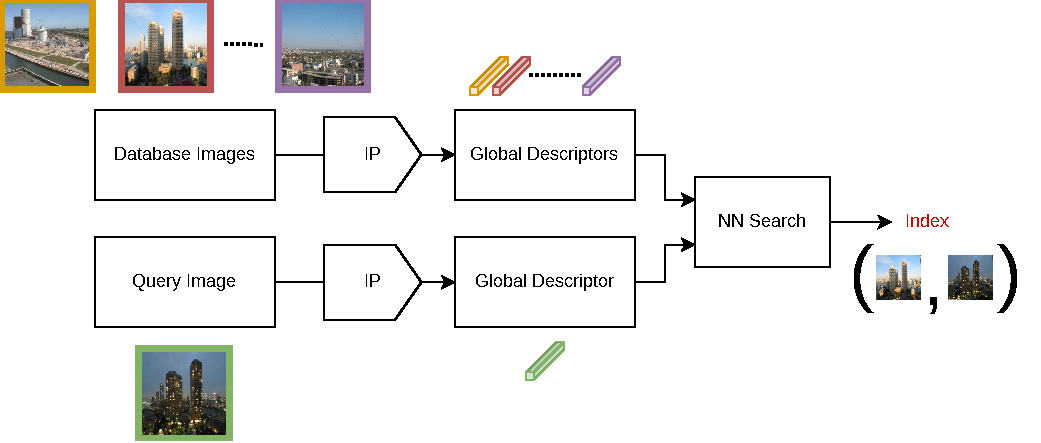
\includegraphics[width=\textwidth]{image_retrieval_system.pdf}
    \caption{Image Retrieval Systems}
    \small
        An Image Processing (IP) algorithm builds \emph{global
        descriptors} from input images. A nearest neighbor search
        takes a query descriptor and a set of global database
        descriptors, and it returns the database descriptor that is
        closest to the query descriptor (as index in set).
    \label{fig:ir_vpr_system}
\end{figure}

A typical Image Retrieval (IR) system is illustrated in
\cref{fig:ir_vpr_system}. The \emph{image processing} stage extracts a
single, unique descriptor that captures the overall visual
characteristics of the entire input image. From a database of
representative images (and their known locations), the image
processing pipeline first builds a database of global descriptors.
Given $N_d$ images of shape $C, H, W$ each (where $H, W$ is the size
of the image and $C$ is the number of channels - 3 for RGB, 1 for
greyscale), we apply the following steps to each image

\begin{enumerate}
    \item \emph{Extract} visual context: This summarizes the visual
    content in an image, yielding descriptors of shape $N, d_p$ (where
    $N$ is the number of descriptors and $d_p$ is the dimensionality).
    There are two main techniques to creating image descriptors for
    extracting visual context of an image:
    \begin{enumerate}
        \item \emph{Local Feature-based}: Identify and describe
        distinctive local features within an image, like corners,
        edges, or blobs. These features are known as keypoints, and
        each keypoint has a corresponding descriptor capturing its
        specific visual characteristics.
        \item \emph{Global Context-based}: Extract descriptors that
        directly represents the entire image. Unlike local
        feature-based methods, they do not rely on identifying and
        describing individual keypoints. Instead, these techniques may
        process the image in different ways, including dividing it
        into smaller overlapping or non-overlapping patches, to
        capture the global visual properties. This allows them to
        capture characteristics such as color distribution, texture
        patterns, and spatial relationships between image elements.
    \end{enumerate}
    \item \emph{Aggregate} descriptors: The previous step yields
    multiple descriptors (keypoints or patches), this step creates a
    single descriptor representing the entire image.  This is usually
    accomplished through clustering and creating histograms. We get
    a $d$-dimensional \emph{global} descriptor per image.
\end{enumerate}

Ideally, global descriptors of similar images (taken from nearby or
same places) should exhibit greater similarity compared to those from
dissimilar images. These descriptors are stored in the memory of the
system. When presented with a query image, the system extracts its
descriptor and performs a nearest-neighbor (NN) search within the
database, retrieving the most similar descriptors and their
corresponding images. In some cases, the system may return multiple
top-k matching image entries. The downstream fine localization task
takes the query image, database image(s) with location(s), and the
registered map to further localize the query in the map.

\paragraph{Mathematical Formulation}
Let 
\begin{math}
    \mathbf{I}_{\textbf{DB}} = \left\{ \mathbf{I}_{DB}[1], 
            \mathbf{I}_{DB}[2], \dots , \mathbf{I}_{DB}[N_d] \right\}
\end{math}
be a set of database images (where $\mathbf{I}_{DB}[i] \in
\mathbb{R}^{C, H, W}$ and $\mathbf{I} \in \mathbb{R}^{N_d, C, H, W}$)
and 
\begin{math}
    \mathbf{D}_{\textbf{DB}} = \left\{ \mathbf{d}_{DB}[1], 
            \mathbf{d}_{DB}[2], \dots, \mathbf{d}_{DB}[N_d] \right\}
\end{math}
be the corresponding global descriptors obtained using
$\mathbf{d}_{DB}[i] = \textrm{GD}(\mathbf{I}_{DB}[i])$ (where
$\mathbf{d}_{DB}[i] \in \mathbb{R}^{d}$ and $\mathbf{D}_{\textbf{DB}} 
\in \mathbb{R}^{N_d, d}$) and where $\textrm{GD}: \mathbb{R}^{C, H, W}
\rightarrow \mathbb{R}^d$ is comprised of the steps above (extract and
aggregate).

A query image $\mathbf{I}_q \in \mathbb{R}^{C, H, W}$ is passed
through the same pipeline $\textrm{GD}(\bullet)$ to obtain its global
descriptor $\mathbf{d}_q = \textrm{GD}(\mathbf{I}_q)$ (where
$\mathbf{d}_q \in \mathbb{R}^{d}$). The nearest neighbor search to
retrieve the top-k most similar database descriptors is done as
follows

\begin{equation}
    \mathbf{S}_{u} = \left\{ \underbrace{
        \textrm{sim}\left ( \mathbf{d}_{DB}[1], \mathbf{d}_q \right ),
        \textrm{sim}\left ( \mathbf{d}_{DB}[2], \mathbf{d}_q \right ), 
        \dots, \textrm{sim}\left ( \mathbf{d}_{DB}[N_d], 
                \mathbf{d}_q \right ) 
        }_{\textup{Similarity Scores}} \right\}
\end{equation}

\begin{equation}
    \mathbf{P} = \textrm{argsort}(\mathbf{S}_{u}, 
                    \textrm{descending})
\end{equation}

\begin{equation}
    \mathbf{V}_{\textup{top-k}} = \mathbf{P}[1:k]
\end{equation}

Where $\mathbf{S}_{u} \in \mathbb{R}^{N_d}$ is a set of unordered
distances between the query and each database descriptor calculated
using a similarity function $\textup{sim}: \left ( \mathbb{R}^d,
\mathbb{R}^d  \right ) \rightarrow \mathbb{R}$ which is a metric like
cosine distance (0 for no similarity and 1 for high similarity). The
$\textrm{argsort}(\bullet, \bullet)$ function takes a set and the
order (\texttt{ascending} or \texttt{descending}) and returns a list
of indices $\mathbf{P} \in \mathbb{N}^{N_d}$ corresponding to the
order. For instance, for \texttt{descending} order,
$\mathbf{S}_u[\mathbf{P}[1]]$ is the largest value in $\mathbf{S}_u$,
$\mathbf{S}_u[\mathbf{P}[2]]$ is the second largest value in
$\mathbf{S}_u$, and so on until $\mathbf{S}_u[\mathbf{P}[N_d]]$ is the
smallest value in $\mathbf{S}_u$. We use indices instead of similarity
values as we're interested in finding the closest database images and
not their similarity scores. We then take the first $k$ values to get
the indices $\mathbf{V}_{\textup{top-k}} \in \mathbb{N}^k$ of the
top-k most similar database images.

\subsubsection{Creating Image Descriptors}

Typically, image descriptors are constructed from local features, as
this approach enables focusing on informative regions within an image.
However, recent advancements in computational power have facilitated
the use of the entire image content (all image patches) for descriptor
creation.

\paragraph{Local Feature Methods} locate and describe keypoints in an
image. These could be manually defined conventional methods like SIFT
\cite{Lowe2004DistinctiveIF}, SURF \cite{Bay2006SURFSU}, BRIEF
\cite{Calonder2010BRIEFBR}, ORB \cite{Rublee2011ORBAE}, AKAZE
\cite{Alcantarilla2013FastED, Alcantarilla2012KAZEF}, etc. or features
that are learned like FAST \cite{Rosten2006MachineLF,
Rosten2008FasterAB}, LIFT \cite{Yi2016LIFTLI}, DELF
\cite{Noh2016LargeScaleIR}, SuperPoint \cite{DeTone2017SuperPointSI},
L2-Net \cite{Tian2017L2NetDL}, R2D2 \cite{Revaud2019R2D2RA}, D2-Net
\cite{Dusmanu2019D2NetAT}, OriNet \cite{Laguna2019KeyNetKD,
Mishkin2017RepeatabilityIN, Mishchuk2017WorkingHT}, etc. A thorough
benchmarking of these algorithms towards image matching is presented
in \cite{Jin2020ImageMA}. These methods take an image $\mathbf{I} \in
\mathbb{R}^{C, H, W}$ and return keypoints $\mathbf{K} \in
\mathbb{R}^{N_k, 2}$ (a list of locations of interest $\{\dots,(h_i,
w_i),\dots\}$) and descriptors $\mathbf{D}_{k} \in \mathbb{R}^{N_k,
d_k}$, where $N_k$ is the number of keypoints and $d_k$ is the
dimensionality of the descriptor (for example, $d_k = 128$ for SIFT).

\paragraph{Global Context through Image Patches} divides the input
image into a set of patches and processes them individually. It takes
an image $\mathbf{I} \in \mathbb{R}^{C, H, W}$ and breaks it uniformly
into patches of shape $\mathbf{G} \in \mathbb{R}^{N_p, C, s_h, s_w}$
where $N_p = n_h \times n_w$ is the number of patches ($n_h$ along the
height and $n_w$ along the width), each patch is of shape $s_h, s_w$
($s_h = s_w = 16$ for ViT). If the patches are non-overlapping and
uniform, then $H = s_h \times n_h$ and $W = s_w \times n_w$.
$\mathbf{G}$ can be reshaped into $\mathbf{D}_p \in \mathbb{R}^{N_p,
d_p}$ where $d_p = C \times s_h \times s_w$.

\paragraph{Bag of Visual Words (BoVW)} \cite{Sivic2003VideoGA}
approach represents an image as a histogram of visual words. Given a
database of images denoted by $\mathbf{I}_{\textbf{DB}}$, it first
extracts local image features using methods like those mentioned
previously. These features are then encoded into corresponding
descriptors, denoted by $\mathbf{V}_{\textbf{DB}} \in
\mathbb{R}^{N_{total}, d}$, where $N_{total}$ represents the total
number of descriptors extracted from all $N_d$ database images. These
$N_{total}$ descriptors are then clustered into $k$ clusters using a
technique like k-means clustering. The centers of these clusters form
the \emph{vocabulary}. For each image, the BoVW approach counts the
number of features belonging to each cluster, essentially building a
histogram. This histogram representation is typically limited to the
top-n most frequent vocabulary terms. This image processing pipeline
provides a histogram representation for each image in the database.
When a new image is considered, its histogram is compared against the
histograms of stored database images using metrics like chi-squared
distance, histogram intersection, cosine distance, or other nearest
neighbor approaches. This is the vision equivalent of Bag-of-Words
(BOW) from NLP for language and document retrieval.

Building upon the standard BoW, the \emph{spatial BoW} approach
incorporates spatial information. It divides the image into smaller
regions and independently applies BoW to each region. This creates a
local vocabulary for each region, capturing the presence of visual
words within specific image areas. The final image representation
combines information from all regional BoW histograms, potentially
including the location of each region within the image.

To improve efficiency for real-time applications, some approaches
convert descriptors to \emph{binary} strings using a thresholding
technique on the histogram values. Alternatively, certain local
feature extraction methods inherently produce binary descriptors. This
binary representation enables faster comparisons during the matching
stage. 

\emph{Hierarchically structured} vocabularies can also be constructed
using clustering methods. \cite{Nistr2006ScalableRW} propose a method
where each cluster in a hierarchical structure is further partitioned,
and a clustering technique like k-means is applied recursively at each
level. This approach facilitates a coarse-to-fine vocabulary creation
suitable for long-term operations. DBoW2 \cite{GlvezLpez2012BagsOB}
uses this technique with binary descriptors while also leveraging it
for loop detection.

\paragraph{VLAD \cite{Arandjelovi2013AllAV, Jgou2010AggregatingLD}}
Vector of Locally Aggregated (VLAD) descriptor is constructed by
following these steps:

\begin{enumerate}
    \item \emph{Feature Extraction}: Local features descriptors such
        as SIFT (or RootSIFT \cite{Arandjelovi2012ThreeTE}) are
        extracted from the image.
    \item \emph{Cluster Assignment}: Each descriptor is assigned to
        its closest cluster in a pre-defined vocabulary of size $k$.
    \item \emph{Residual Accumulation}: For each cluster, the
        residuals are calculated. These residuals are vector
        differences between the assigned descriptors and the cluster
        centers. The residuals are then accumulated (added) to obtain
        a 128-d vector (same dimensionality as descriptor used) per
        cluster.
    \item \emph{VLAD Descriptor Formulation}: Finally, the $128-d$
        residuals across all $k$ clusters are concatenated to form a
        single $k \times 128$ dimensional vector which is the VLAD
        vector.
\end{enumerate}

We normalize the accumulated cluster residuals before concatenation
(known as intra-norm) and normalize the final concatenated result to
prevent bias towards a small subset of clusters and to effectively
utilize the entire vocabulary. The vocabulary is constructed by
extracting descriptors across all the database images and clustering
them using a method like k-means. Since the cluster assignment of VLAD
is non-differentiable, it cannot directly be used for training.

Mathematically, given an image $\mathbf{I} \in \mathbb{R}^{C, H, W}$,
we extract its keypoints $\mathbf{K} \in \mathbb{R}^{N_k, 2}$ and
descriptors $\mathbf{D} \in \mathbb{R}^{N_k, d_k}$. We have
$\mathbf{C} \in \mathbb{R}^{K, d_k}$ as the vocabulary ($K$ cluster
centers, each $d_k$ dimensional). We compute a residual matrix
$\mathbf{V} \in \mathbb{R}^{K, d_k}$ as follows

\begin{equation}
    \mathbf{V}[k, j] = \sum_{i=1}^{N_k} \left[ \alpha \left (
            \mathbf{D}[i], k \right ) \left ( 
                \mathbf{D}[i, j] - \mathbf{C}[k, j] \right ) \right]
\end{equation}

Where $\mathbf{V}[k, j] \in \mathbb{R}$ is the residual for the $k$-th
cluster center's $j$-th dimension, $\alpha:(\mathbb{R}^{d_k},
\mathbb{N}) \rightarrow \{0, 1\}$ takes in the descriptor and cluster
index; and returns 1 if the descriptor belongs to the cluster (the
given cluster is the closest to the descriptor) and 0 otherwise. The
matrix $\mathbf{V}$ is normalized along $d_k$ (each of $K$ rows, which
is a $d_k$-dimensional vector, is normalized) for intra-normalization.
It is then reshaped (flattened) to a vector $\mathbf{v} \in
\mathbb{R}^{K \times d_k}$ and then normalized (same shape). This
final vector $\mathbf{\hat{v}} = \left\| \mathbf{v} \right\|_2$ is the
VLAD vector.

The cluster centers $\mathbf{C} \in \mathbb{R}^{K, d_k}$ are obtained
by applying a clustering technique like k-means clustering to the
descriptors from database images. We start with a set of database
images $\mathbf{I}_\textbf{DB} = \{\mathbf{I}_1, \mathbf{I}_2, \cdots,
\mathbf{I}_{N_d}\}$, where $\mathbf{I}_i \in \mathbb{R}^{C, H, W}$ is
a database image, and extract its corresponding local feature
descriptors $\mathbf{D}_{\textbf{kdb}} = \{\mathbf{D}_1, \mathbf{D}_2,
\cdots, \mathbf{D}_{N_d} \}$ where $\mathbf{D}_i \in \mathbb{R}^{N_i,
d_k}$ is the list of descriptors for image $\mathbf{I}_i$ (each image
might have a different number of descriptors). These descriptors are
stacked along $N_i$ dimension to give $\mathbf{D}_{all} \in
\mathbb{R}^{N_{total}, d_k}$ (where $N_{total} = \sum_i N_i$). These
$N_{total}$ descriptors are clustered into $K$ clusters giving the
cluster centers $\mathbf{C} \in \mathbb{R}^{K, d_k}$.

\paragraph{NetVLAD \cite{Arandjelovi2015NetVLADCA}} is a
differentiable version of VLAD. VLAD has two non-differentiable steps:
\emph{clustering} for fitting on database images (descriptors) and
cluster \emph{assignment} during construction of VLAD, denoted as
$\alpha(\bullet, \bullet)$ above. NetVLAD uses the following cluster
assignment instead

\begin{equation}
    \tilde{\alpha} \left( \mathbf{d}_i, \mathbf{c}_k \right) = 
        \frac{e^{-\lambda 
            \left\| \mathbf{d}_i - \mathbf{c}_k \right\|_2^2}}
        {\sum_{k'} e^{-\lambda 
            \left\| \mathbf{d}_i - \mathbf{c}_{k'} \right\|_2^2}}
\end{equation}

Where $\mathbf{d}_i = \mathbf{D}[i] \in \mathbb{R}^{d_k}$ is the
$i$-th descriptor in the image and $\mathbf{c}_k = \mathbf{C}[k] \in
\mathbb{R}^{d_k}$ is the $k$-th cluster center. The above equation can
be simplified further

\begin{align*}
    \left\| \mathbf{d}_i - \mathbf{c}_k \right\|_2^2 &= \sum_j \left(
        \mathbf{d}_i[j] - \mathbf{c}_k[j]\right)^2 = \sum_j \left[
        \mathbf{d}_i[j]^2 + \mathbf{c}_k[j]^2 
            - 2\mathbf{d}_i[j]\mathbf{c}_k[j]\right] \\
        &= \left\| \mathbf{d}_i^2 \right\|_1 + 
            \left\| \mathbf{c}_k^2 \right\|_1 - 
            2 \mathbf{d}_i \cdot \mathbf{c}_k \\
    e^{-\lambda\left\| \mathbf{d}_i - \mathbf{c}_k \right\|_2^2} &=
        e^{2\lambda \mathbf{d}_i \cdot \mathbf{c}_k} \cdot
        e^{-\lambda \left\| \mathbf{d}_i^2 \right\|_1} \cdot
        e^{-\lambda \left\| \mathbf{c}_k^2 \right\|_1} \\
    e^{-\lambda\left\| \mathbf{d}_i - \mathbf{c}_{k'} \right\|_2^2} &=
        e^{2\lambda \mathbf{d}_i \cdot \mathbf{c}_{k'}} \cdot
        e^{-\lambda \left\| \mathbf{d}_i^2 \right\|_1} \cdot
        e^{-\lambda \left\| \mathbf{c}_{k'}^2 \right\|_1} \\
    \tilde{\alpha} \left( \mathbf{d}_i, \mathbf{c}_k \right) &= 
        \frac{e^{-\lambda 
            \left\| \mathbf{d}_i - \mathbf{c}_k \right\|_2^2}}
        {\sum_{k'} e^{-\lambda 
            \left\| \mathbf{d}_i - \mathbf{c}_{k'} \right\|_2^2}} =
        \frac{e^{2\lambda \mathbf{d}_i \cdot \mathbf{c}_k} \cdot
            e^{-\lambda \left\| \mathbf{d}_i^2 \right\|_1} \cdot
            e^{-\lambda \left\| \mathbf{c}_k^2 \right\|_1}}{\sum_{k'}
            e^{2\lambda \mathbf{d}_i \cdot \mathbf{c}_{k'}} \cdot
            e^{-\lambda \left\| \mathbf{d}_i^2 \right\|_1} \cdot
            e^{-\lambda \left\| \mathbf{c}_{k'}^2 \right\|_1}} \\
        &= \frac{e^{2\lambda \mathbf{d}_i \cdot \mathbf{c}_k -
                \lambda \left\| \mathbf{c}_k^2 \right\|_1}}{\sum_{k'}
                e^{2\lambda \mathbf{d}_i \cdot \mathbf{c}_{k'} -
                \lambda \left\| \mathbf{c}_{k'}^2 \right\|_1}}
        = \frac{e^{\mathbf{w}_k^T \mathbf{d}_i + b_k}}{\sum_{k'}
        e^{\mathbf{w}_{k'}^T \mathbf{d}_i + b_{k'}}}
\end{align*}

The final VLAD residual matrix becomes

\begin{equation}
    \mathbf{V}[k, j] = \sum_{i=1}^{N_k} \left[ 
        \frac{e^{\mathbf{w}_k^T \cdot \mathbf{d}_i + b_k}}{\sum_{k'}
            e^{\mathbf{w}_{k'}^T \cdot \mathbf{d}_i + b_{k'}}}
        \left ( \mathbf{D}[i, j] - \mathbf{C}[k, j] \right ) \right]
\end{equation}

Where $\{\mathbf{w}_k \in \mathbb{R}^{d_k}\}$, $\{b_k \in
\mathbb{R}\}$, and $\mathbf{C} \in \mathbb{R}^{K, d_k}$ are trainable
parameters. Conventionally, the descriptors $\mathbf{D} \in
\mathbb{R}^{N_k, d_k}$ are obtained as dense features from a CNN
backbone.

\paragraph{GeM Pooling \cite{Radenovic2017FineTuningCI}} uses
generalized mean pooling over image descriptors $\mathbf{D} \in
\mathbb{R}^{N_k, d_k}$ and yields a vector $\mathbf{f}_G \in
\mathbb{R}^{d_k}$ where each element is given by

\begin{equation}
    \mathbf{f}_G[j] = \left( \frac{1}{N_k} \sum_{i=1}^{N_k} 
        \left(\mathbf{D}[i, j]\right)^{p_k}\right)^{\frac{1}{p_k}}
\end{equation}

An advantage of GeM pooling is that the dimension of the output
descriptor is $d_k$, whereas it is $K \times d_k$ for VLAD. This
facilitates storing more of them on limited memory.

\paragraph{Other Pooling Methods} include max-pooling ,also called
\emph{MAC} (Maximum Activations of Convolutions) vector
\cite{Razavian2014VisualIR, Tolias2015ParticularOR} given by
$\mathbf{f}_M \in \mathbb{R}^{d_k}$ and average-pooling, also called
SPoC (Sum-Pooled Convolution) features \cite{Babenko2015AggregatingLD}
given by $\mathbf{f}_A \in \mathbb{R}^{d_k}$. These are defined below

\begin{align}
    \mathbf{f}_M[j] &= \underset{i}{\mathrm{max}} \, \mathbf{D}[i, j]
    &
    \mathbf{f}_A[j] &= \frac{1}{N_k} \sum_{i=1}^{N_k} \mathbf{D}[i,j]
\end{align}

\subsubsection{Other Approaches to VPR}

While traditional approaches to VPR often rely on features extracted
from trained CNN backbones \cite{Sarlin2018FromCT}, this thesis
focuses on leveraging foundation models for this task.  

Other areas of exploration in VPR include the use of sequential
descriptors \cite{Garg2021SeqNetLD, Garg2021SeqMatchNetCL,
Xu2018SequentialVV}, low-resolution image training
\cite{Khaliq2022MultiResNetVLADAP}, and visual semantics
\cite{Garg2018LoSTAP}. Techniques like mesh-based localization
\cite{Panek2022MeshLocMV}, direct 2D-3D matching
\cite{Sattler2011FastIL}, change-based VPR \cite{Garg2020DeltaDC},
hierarchical 3D descriptors \cite{Du2020DH3DDH}, novel pooling methods
(like SuperGlobal \cite{Shao2023GlobalFA}), and cross-device queries
\cite{Huang2023360LocAD} are also being investigated, along with the
development of sequential SLAM pipelines \cite{Milford2012SeqSLAMVR}.

